\documentclass[../main.tex]{subfiles}

\begin{document}
	\pagebreak
	\rhead{Cameron Eadie}
\section{Literature Review - UFOs} \label{UFO_Lit_Review}
Several papers have been produced by CERN describing the UFO problem, and attempts to identify the UFOs through simulations.
The majority of UFO events occur in the vertical plane, described by Nebot del Busto et al \cite{nebot_vertical}.
The initial theory was that this vertical characteristic is due to the UFOs falling under the effects of gravity from the top surface of the beam screen (see figure \ref{fig:UFO_Falling}).\\

\begin{figure}[ht]
	\centering
	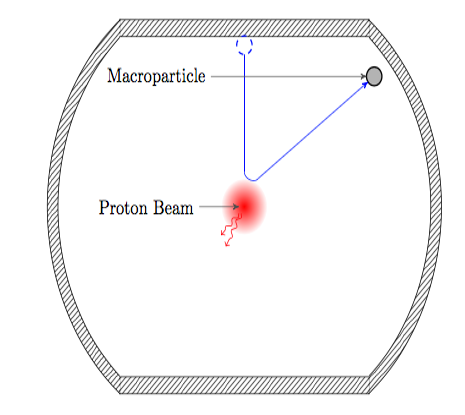
\includegraphics[width=0.6\textwidth]{UFO_Falling.png}
	\caption{UFO Depicted Falling into the Proton Beam (Figure - Tom O'Connor)}
	\label{fig:UFO_Falling}
\end{figure}

It was noted by Baer et al \cite{baer_accel} in 2011, however, that the accelerations of particles from the surfaces would have to be $\approx \SI{3500}{\metre\per\second\squared}$ given the shortest delay after injection of the first UFO events.
This suggested that the acceleration of the UFOs was not due to gravity alone, but that they must be accelerating significantly faster, either due to electric attraction or forces applied by the magnetic fields.
These calculations were based on events near the Injection Kicker Magnets (MKIs) which inject the beam into the LHC, and so either is possible.
The same paper also noted two noteworthy facts.
Firstly, the impact of UFO events in the arc sections increases significantly with beam energy, and this means that they will have a significant effect on higher energy operation.
This also suggests that higher energies correlate to greater levels of attraction of UFOs to the beam.
Secondly, there were significantly higher numbers of events near the MKIs than anywhere else in the LHC.\\

\begin{figure}[ht]
	\centering
	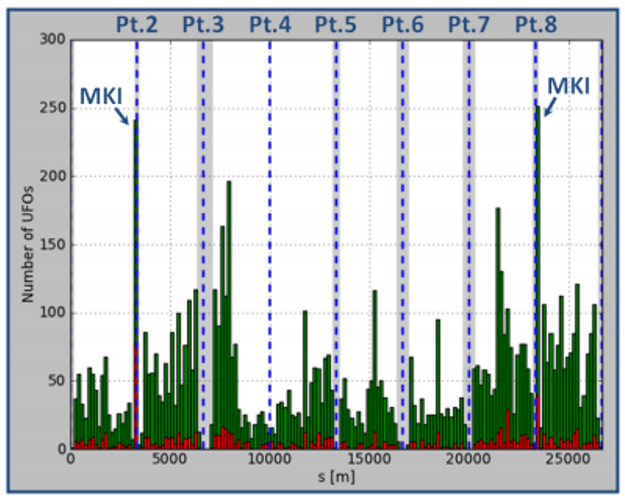
\includegraphics[width=0.6\textwidth]{UFO_Spatial_Distribution.png}
	\caption{Spatial Distribution of 7784 UFO Events at \SI{3.5}{\tera\electronvolt} Between April and October 2011, Showing  Clear Peaks at the MKIs \cite{baer_distributions}}
\end{figure}   

Another paper by Baer et al \cite{baer_mki} investigated the MKI UFOs in more detail.
It concluded that the most likely source of these UFOs were the Al$_{2}$O$_{3}$ ceramic tubes in the MKIs.
A nitrogen flush of a removed MKI during the winter of 2010/2011 revealed over 5 million particles on the filter; most of the particles were between \SI{1}{\micro\metre} and \SI{10}{\micro\metre} in size, but some were up to \SI{100}{\micro\metre}.\\

\begin{figure}[ht]
	\centering
	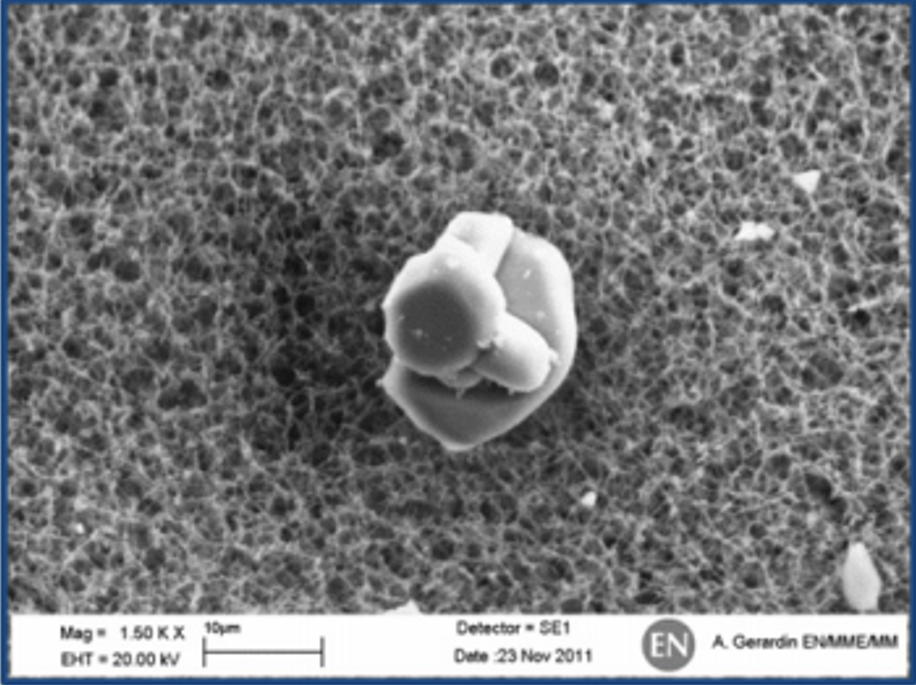
\includegraphics[width=0.6\textwidth]{MKI_UFO.png}
	\caption{UFO Particle from the MKI Flush (about \SI{10}{\micro\metre}) \cite{baer_mki}}
\end{figure}

Energy-dispersive x-ray spectroscopy (EDS) of these particles suggest that the majority of the particles consisted of Al and O.
There were also traces of gold in the EDS spectrum, which would suggest that some of the particles came from the gold-plated RF fingers which are present every \SI{15}{\metre} in the LHC (see figure \ref{fig:RF_Fingers}).
These fingers are in the interconnects between sections, and are made of a copper-beryllium composite.
They act as thermal expansion joints between the sections, required because of the large range of temperature some sections go through.
They are gold-plated to better carry the image currents induced by the proton beam between sections.\\

\begin{figure}[ht]
	\centering
	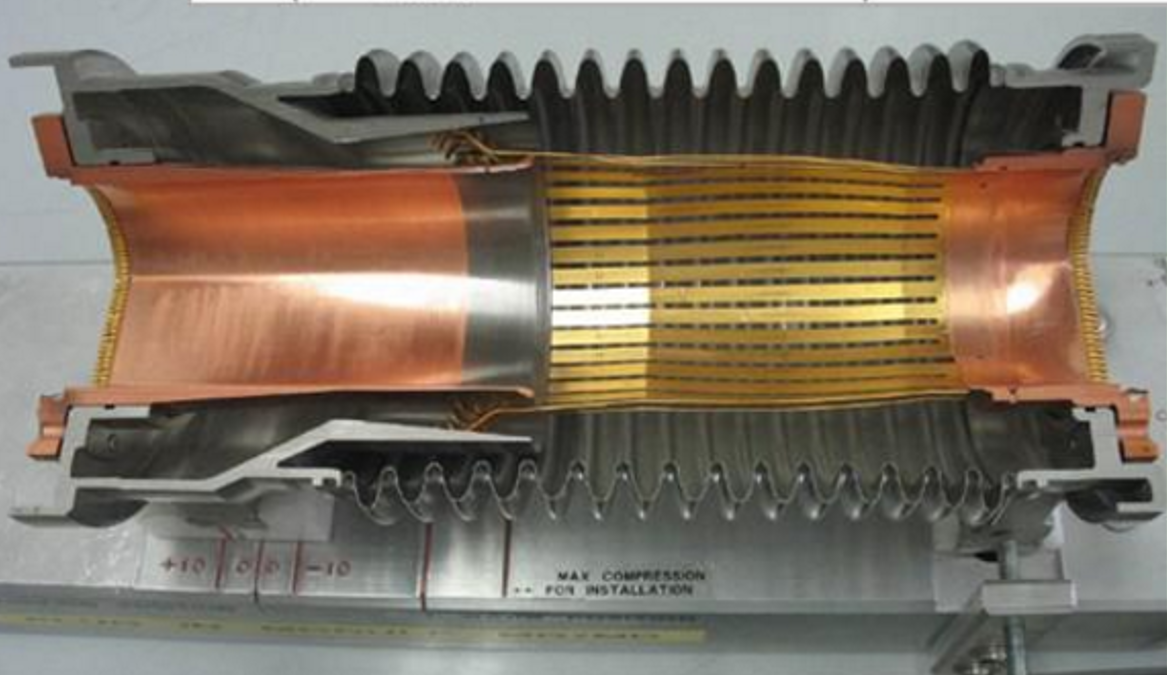
\includegraphics[width=0.8\textwidth]{RF_Fingers.png}
	\caption{Gold-Plated RF Fingers in the Interconnects}
	\label{fig:RF_Fingers}
\end{figure}

It should be noted that there is no viable mechanism by which these MKI UFOs could travel along the length of the LHC, and so the issue of arc UFOs is likely due to a different, more distributed source, such as the RF fingers.
The MKI UFOs are thought to be of a different species of particle to those in the arc sections \cite{grob_ufo}.
During the Long Shutdown of the LHC in 2013/2014, all eight MKIs were upgraded.
The ceramic tubes were better cleaned with water and then with nitrogen flushes until no further significant reduction in the number of macroparticles was noted \cite{barnes_mki}.
This has successfully mitigated the majority of the MKI UFO events.
Along with gold being found in the MKI dust spectrum, scratches have also been observed on the copper surfaces of the beam screen where the RF fingers contact them, due to expansion and contraction.
For this reason gold and copper are strong candidate materials for arc UFOs.
The conductivity of metallic UFOs would also explain the increasing number of events as power is increased, as the proton beam would generate stronger electric fields to attract the UFOs.\\

UFO events decrease over time, seeming to show a clear conditioning effect due to running of the LHC \cite{baer_distributions}.
In 2011 there was a reduction in the average number of events from 10 events per hour to 2 events per hour, with an average over the year of 6 events per hour.
This would suggest that some UFOs are being destroyed or otherwise rendered ineffectual after interacting with the beam.
There is also a marked increase in the number of events directly after a shutdown, suggesting that the shutdowns are introducing some new UFO materials; either due to interacting with the inside of the beam screen, or simply due to expansion, as sections are allowed to warm up and expand.\\

\begin{figure}[ht]
	\centering
	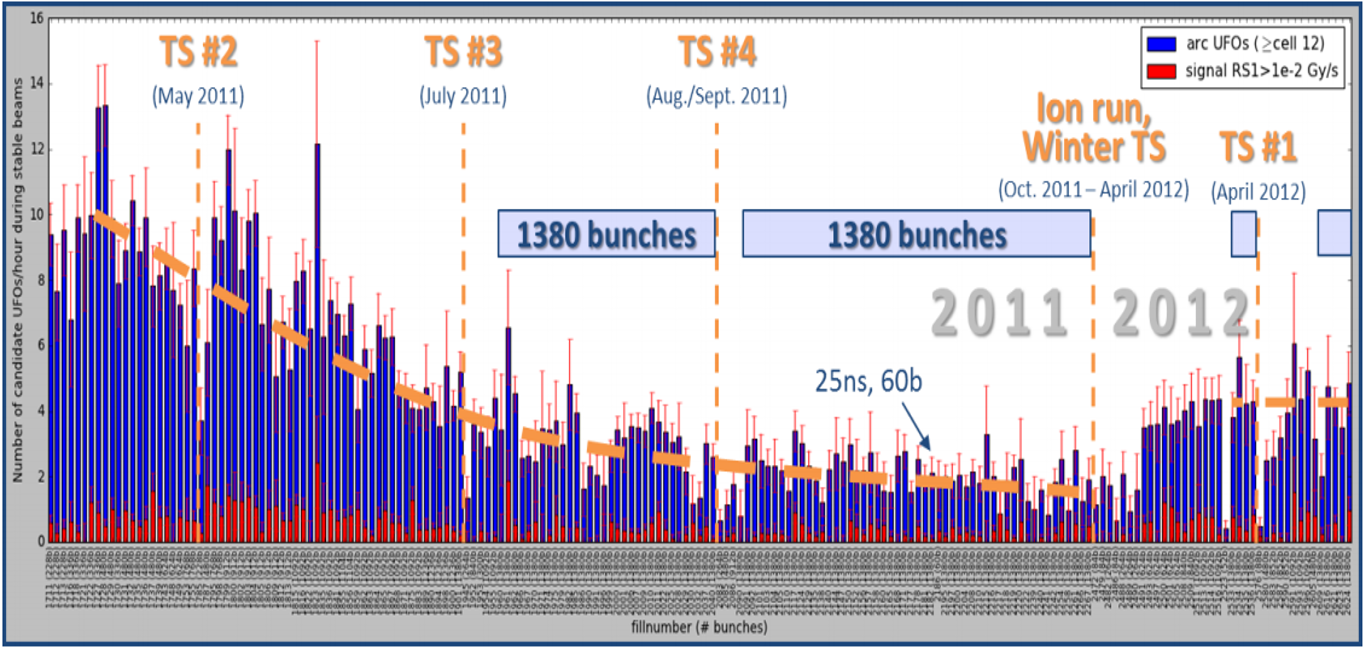
\includegraphics[width=1\textwidth]{UFO_Temporal_Distribution.png}
	\caption{Number of Candidate Arc UFO Events per Hour During Full Energy Stable Beams Between April 2011 and May 2012 \cite{baer_distributions}}
\end{figure}

\end{document}  